\chapter{Konzept}
\section{Aufbau der Software}
    Die im vorherigen Kapitel dargestellten Use-Case Diagramm und den daraus abgeleiteten Anforderungen, werden in diesem Kapitel zum Aufbau einer Architektur verwendet.
    Hierbei wurde zunächst das Systemdiagramm aus dem Use-Case Diagramm abgeleitet.
    
    Die Akteure (\emph{Netwerk-, Systemadministrator} und \emph{Security Auditor}) konnten direkt aus dem Use-Case Diagramm übernommen werden.
    Sie stellen die mit dem System interagierende Nutzer dar und interagieren mit einem Frontend.
    \begin{figure}[h]%h=direkt danach t=top b=bottom
        \centering
        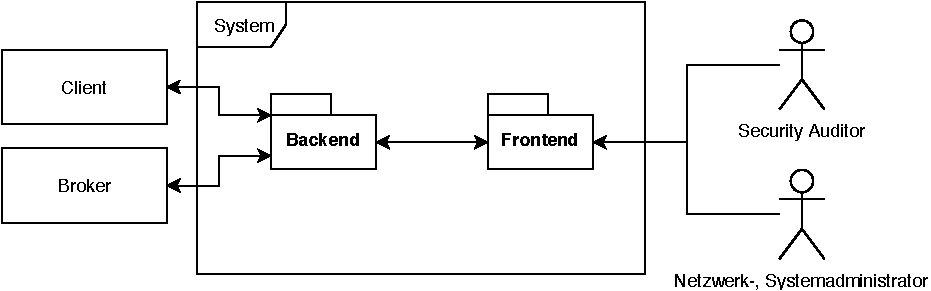
\includegraphics[width=14cm]{tex/bilder/4_konzept/Systemdiagram.pdf}
        \captionof{figure}{Systemdiagramm}
        \label{fig:system_all}
    \end{figure}
    \begin{figure}[h]%h=direkt danach t=top b=bottom
        \centering
        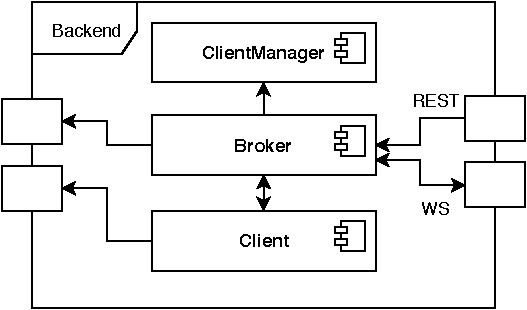
\includegraphics[width=8cm]{tex/bilder/4_konzept/Systemdiagramm_Backend.pdf}
        \captionof{figure}{Komponentendiagramm Backend}
        \label{fig:system_backend}
        \end{figure}
    \begin{figure}[h]%h=direkt danach t=top b=bottom
        \centering
        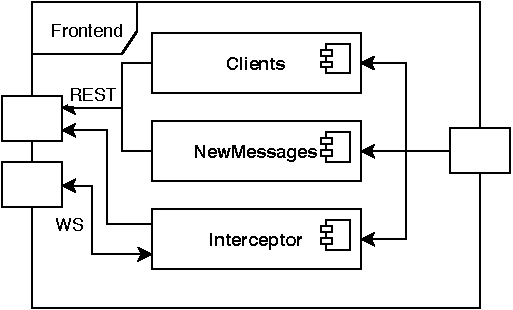
\includegraphics[width=8cm]{tex/bilder/4_konzept/Systemdiagramm_Frontend.pdf}
        \captionof{figure}{Komponentendiagramm Frontend}
        \label{fig:system_frontend}
    \end{figure}

\section{Komponenten}
%Komponentendiagramm

\section{Prozess}
%Aktivitätsdiagramm
%Sequenzdiagramm
